\chapter{Introduction to TI MSP432 Launchpad}

\section{Embedded System Development Platform}

It consists of the \textbf{host system}, that has the cross compiler, linker and source-level debugger.
It also consists of the \textbf{target system}, with debugger, processor, sensors...


There must be connections between the host and target system to \textbf{download program images and
transmit debugger information} between the host debugger and the target debug agent.

\begin{figure}[H]
    \centering
    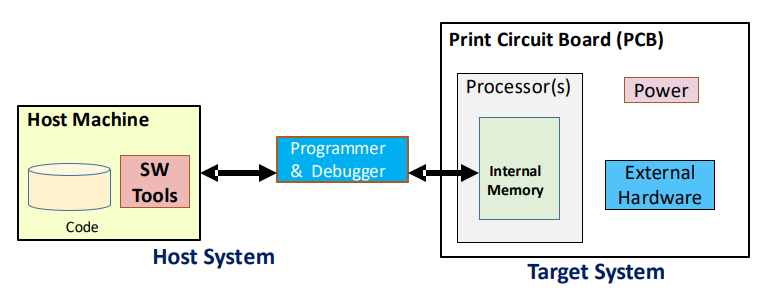
\includegraphics[width=0.8\linewidth]{img/image50.png}
\end{figure}

In the \textit{TI MSP432 Launchpad} the Programmer \& debugger is also inside the target system.

\subsection{Launchpad}
It's a whole Printed Circuit Board (PCB) used as a development kit, allowing you to mess around with the
code and re-flash it each time. When the code is ready for production, and can be burned in a ROM, all
you will need is the processor. Most vendors provide these kits.
\begin{figure}[H]
    \centering
    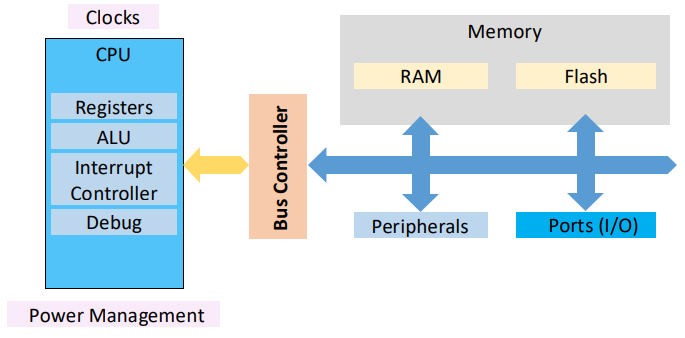
\includegraphics[width=0.7\linewidth]{img/image51.png}
\end{figure}

\section{Microcontroller Components}



\begin{figure}[H]
    \centering
    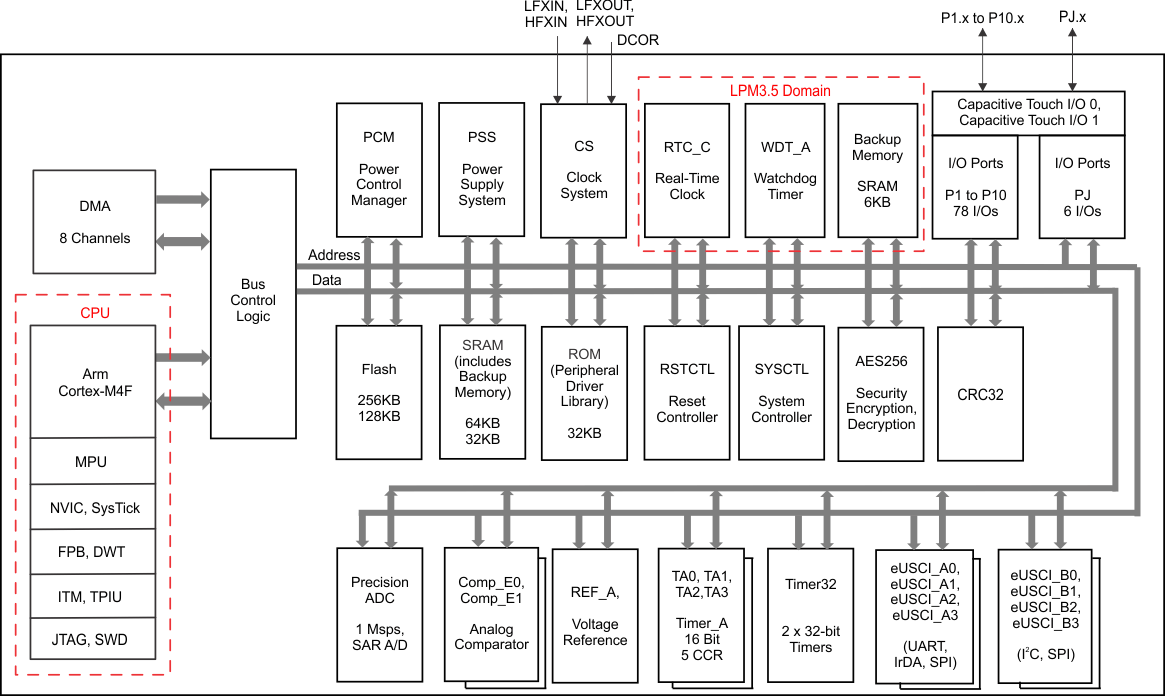
\includegraphics[width=1\linewidth]{img/MSP432P401M-functional-block-diagram.png}
\end{figure}

\begin{figure}[H]
    \centering
    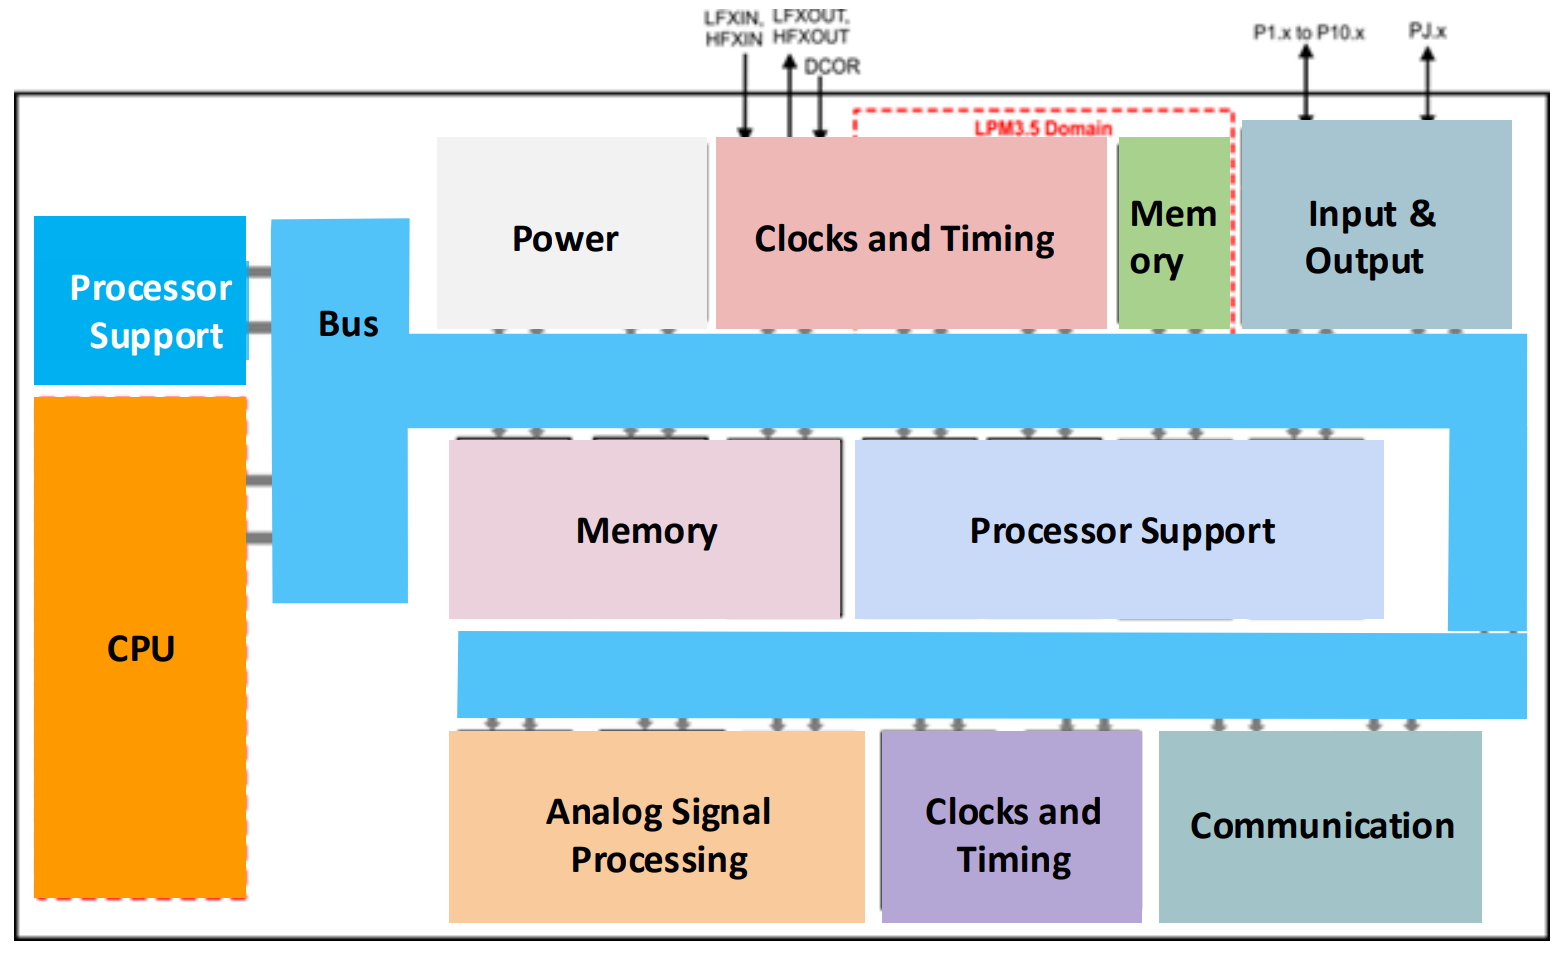
\includegraphics[width=1\linewidth]{img/image53.png}
\end{figure}

\newpage
\subsection{TI-MSP432 microcontroller main features}

\begin{itemize}
    \item[-] \textbf{ARM(r) Cortex(tm)-M4F} processor - Designed for low-power, embedded systems application
    \item[-] MSP stands for Mixed Signals Processing, can read both analogue and digital values
    \item[-] 100-pin microcontroller chip
    \item[-] Peripherals: 256KB on-chip Flash memory for code, 64KB on-chip SRAM for data, large number of on-chip peripherals
\end{itemize}


\subsection{Memory Map in MSP432P401R}

\begin{figure}[H]
    \centering
    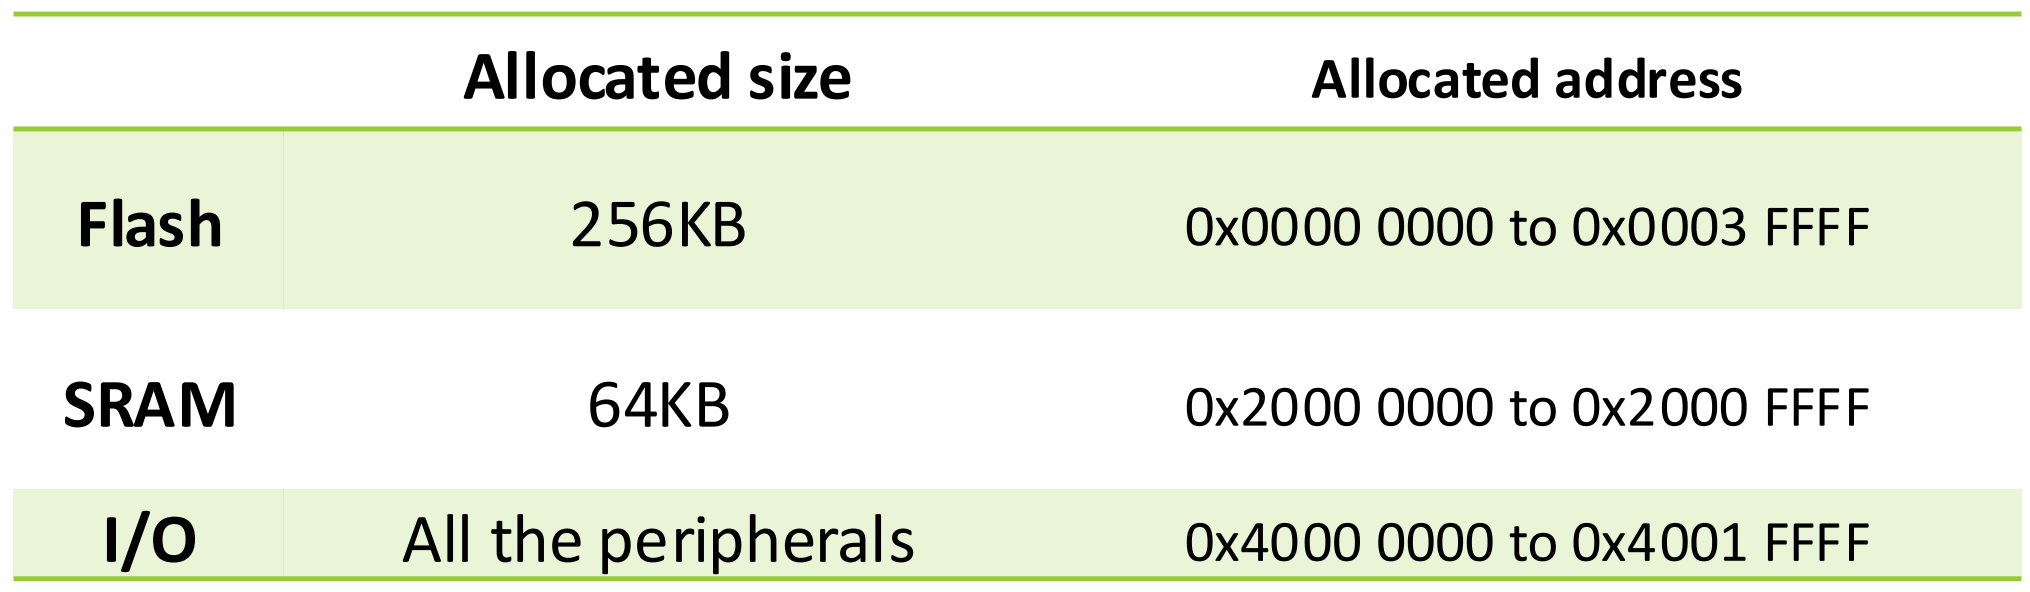
\includegraphics[width=0.6\linewidth]{img/image54.png}
\end{figure}

\section{Running an application on the launchpad}

\textbf{New project:}
    \begin{itemize}
        \item[$\rightarrow$] Create new project
        \item[$\rightarrow$] Select target microcontroller
        \item[$\rightarrow$] Empty project with main.c
        \item[$\rightarrow$] Everything else default
    \end{itemize}
\textbf{Compiling the project:}
    \begin{itemize}
        \item[$\rightarrow$] Rebuild the project
    \end{itemize}
\textbf{Burn/Load the project onto the launchpad:}
\begin{itemize}
        \item[$\rightarrow$] Debug project
    \end{itemize}

    The application runs on bare metal programming, thus there is no OS or external support whatsoever.
You can see all instructions and manipulate memory at will. All you're facing is the actual hardware. We
can see the registers, variables, memory browser, assembly instructions and so on (expressions,
breakpoints...).

\section{Peripherals}


They are external to CPU:

\begin{minipage}{\linewidth}
      \centering
      \begin{minipage}{0.40\linewidth}
            \begin{itemize}
                \item Memory-mapped I/O to configure peripherals
                \item Pointers
                \item Memory Reads/Writes
                \item Use of Bit Manipulation
            \end{itemize}
      \end{minipage}
      \hspace{0.05\linewidth}
      \begin{minipage}{0.35\linewidth}
            \begin{figure}[H]
                \centering
                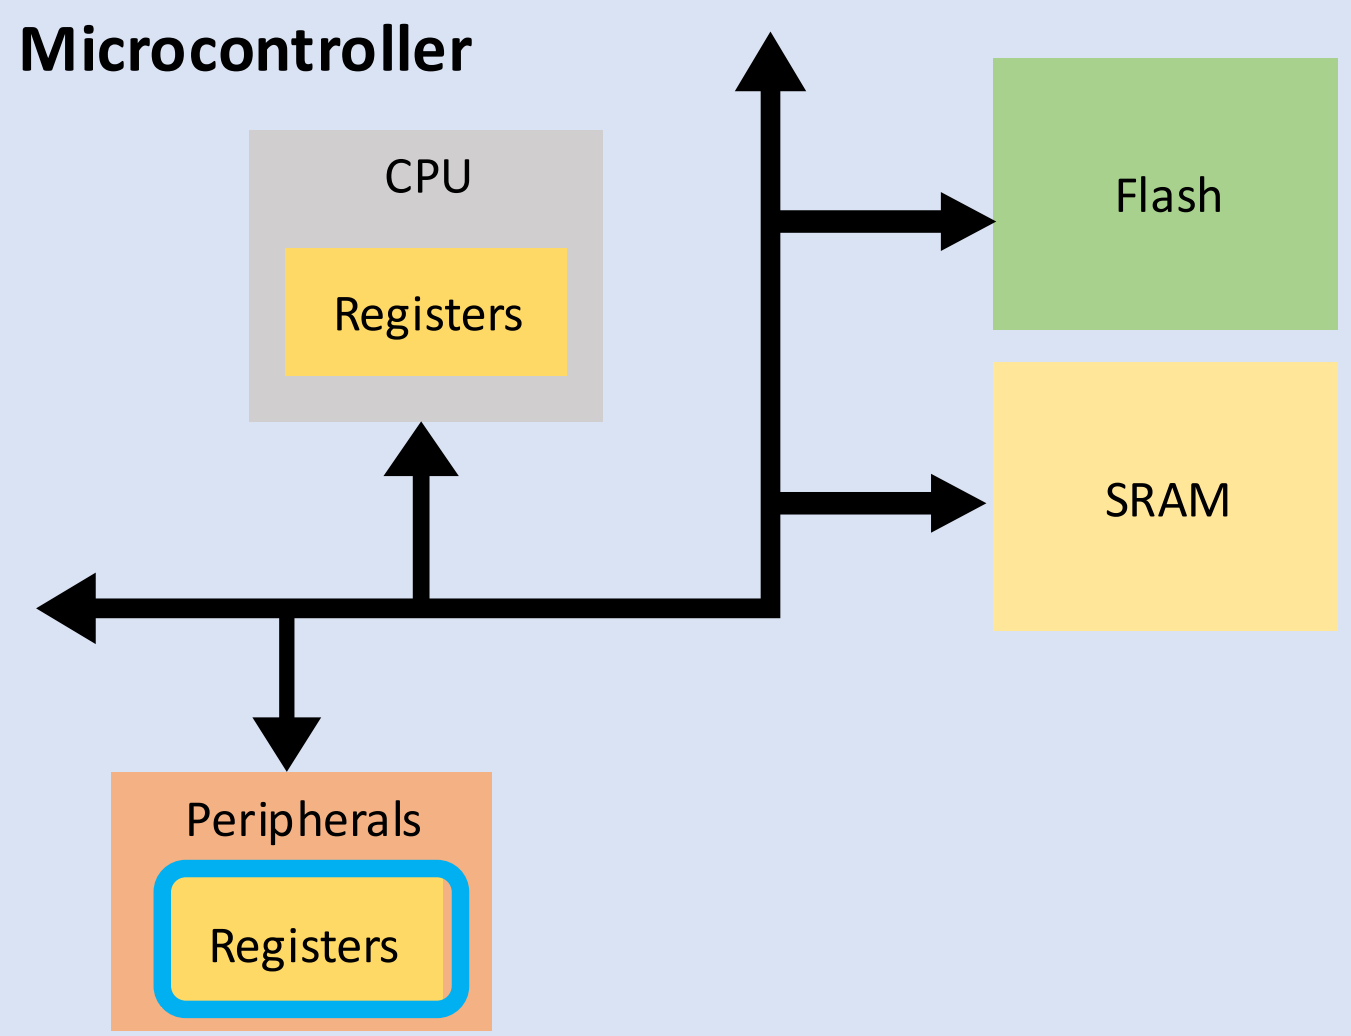
\includegraphics[width=1\linewidth]{img/image55.png}
            \end{figure}
      \end{minipage}
  \end{minipage}








\section{GPIO - Input/Output Systems}

\textbf{GPIO-General Purpose IO}: Pin – physical connection to microcontroller, Port – combination of pins
\textbf{Input/Output}: method to get data in/out of microcontroller

\begin{figure}[H]
    \centering
    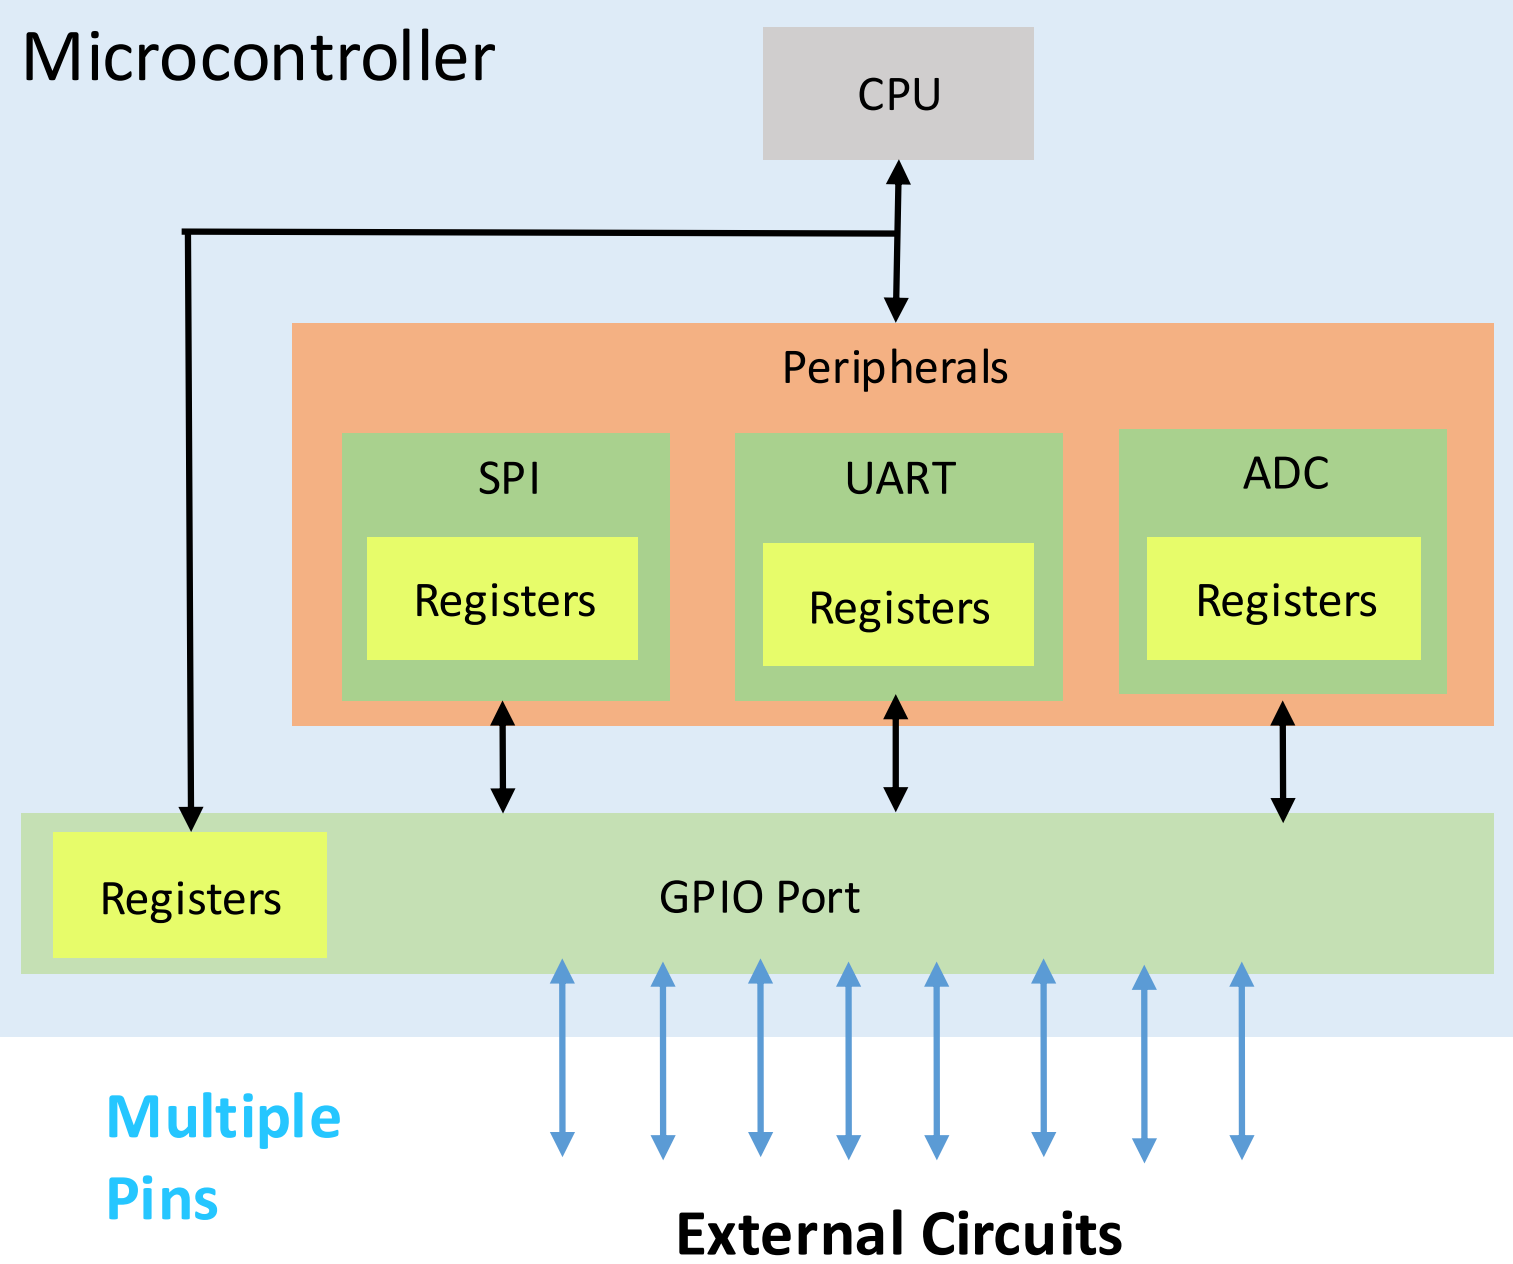
\includegraphics[width=0.5\linewidth]{img/image56.png}
\end{figure}

Pins may have different features, to enable an alternative function, set up the appropriate register

\begin{figure}[H]
    \centering
    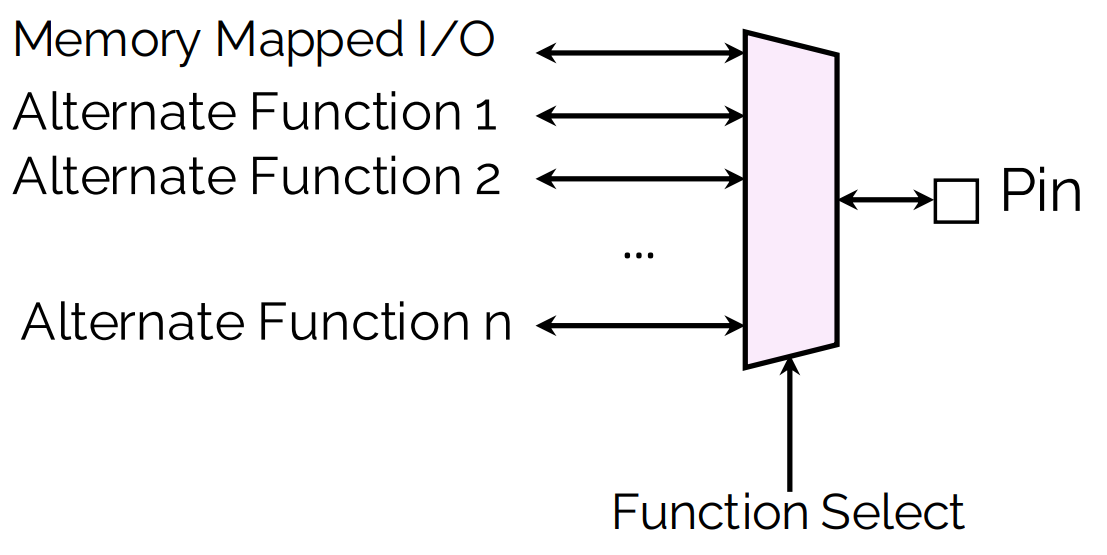
\includegraphics[width=0.5\linewidth]{img/image57.png}
\end{figure}

In the microcontroller, we have two types of I/O:

\begin{itemize}
    \item[] \textbf{General Purpose I/O} (GPIO) - the GPIO ports are used for interfacing devices such as LEDs, switches, LCD, keypad, and so on.
    \item[] \textbf{Special purpose I/O} - These I/O ports have designated function such as ADC (Analog-toDigital), Timer, UART (universal asynchronous receiver transmitter), and so on.
\end{itemize}

The GPIO ports in MSP432 are designated as port P1 to P10 - Simple I/O or Digital I/O ports - and PJ - special function such as crystal oscillator and JTAG connections.

\newpage
\section{Configuring LED}

To \textbf{configure} LED on P1.0

\begin{itemize}
    \item set direction to output: \textbf{P1DIR}
    \item Set P1.0 output to high: \textbf{P1OUT}
\end{itemize}


\begin{figure}[H]
    \centering
    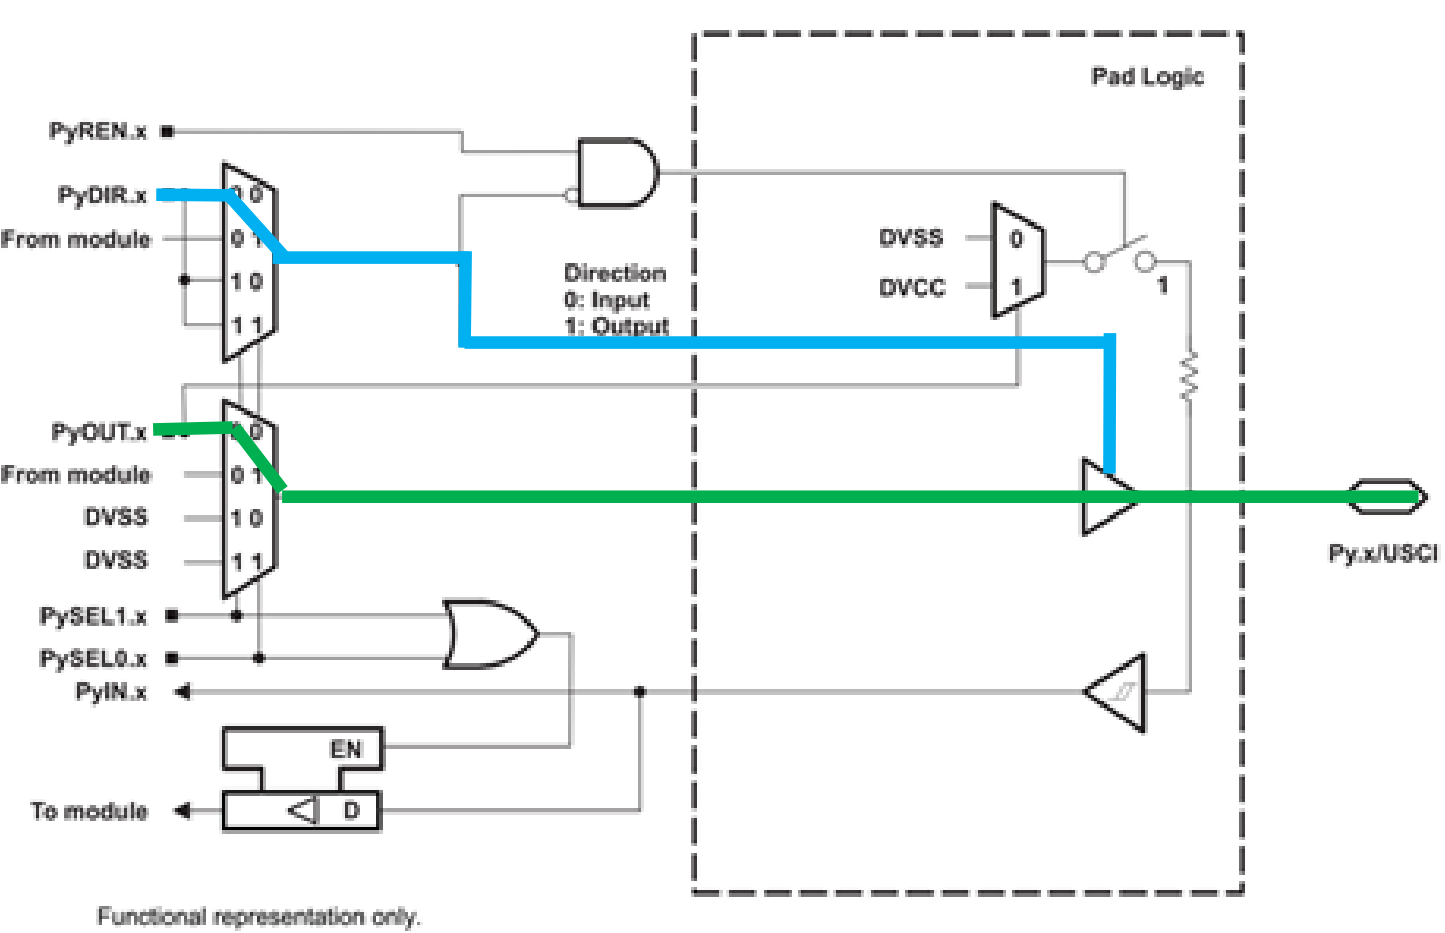
\includegraphics[width=0.7\linewidth]{img/image60.png}
\end{figure}

To\textbf{ turn on} LED, P1.0\_LED1: voltage needs to be a Logical HI (VCC 3.3V).

Also Required to Set Pin to \textbf{I/O Mode} (P1SELx).

\paragraph{Two important registers:} IO Direction Register, \textbf{P1DIR}, IO Output Register, \textbf{P1OUT}.

\subsection{P1DIR Register}

Port Direction Register sets the
pin to:

\begin{itemize}
    \item 0: an input
    \item 1: an output
\end{itemize}

\begin{lstlisting}[language=c++]

    /* Configure P1.0 output */
    P1->DIR |= BIT0; 
\end{lstlisting}


\subsection{P1OUT Register}

Port Output Register sets output to:

\begin{itemize}
    \item 0: Output set to LOW (GND)
    \item 1: Output set to HIGH (VCC)
\end{itemize}

\begin{lstlisting}[language=c++]

    /* Configure P1.0 output */
    P1->DIR |= BIT0;
    /* Set P1.0 HIGH */
    P1->OUT |= BIT0;
\end{lstlisting}

\section{Configure the buttons}

Buttons are connected to P1.1 and P1.34

\begin{lstlisting}[language=c++]

    /* Configure P1.1 as input*/
    P1->DIR = ~BIT1; //BIT0 as output
    /* Select pullup*/
    P1->OUT = BIT1; //BIT0 pulldown
    /* Enable pullup*/
    P1->REN = BIT1; //BIT0 disable
    /* Set as I/O */
    P1->SEL0 = 0;   //general purpose I/O selected
    P1->SEL1 = 0;
    ...
    /* Catch Button Press */
    while (P1->IN & BIT1);
    while (!(P1->IN & BIT1));
    ...
\end{lstlisting}

\subsection{Pull-up and Pull-down Resistors}

If we do not use internal pull-up (or pull-down) resistors, we have a
problem. We need to ensure a known value on the output if a pin is left floating.

We want the switch SW to pull the pin to ground, so we enable the pull-up. The pin value is:

\begin{itemize}
    \item High when SW is not pressed
    \item Low when SW is pressed
\end{itemize}


\begin{figure}[H]
    \centering
    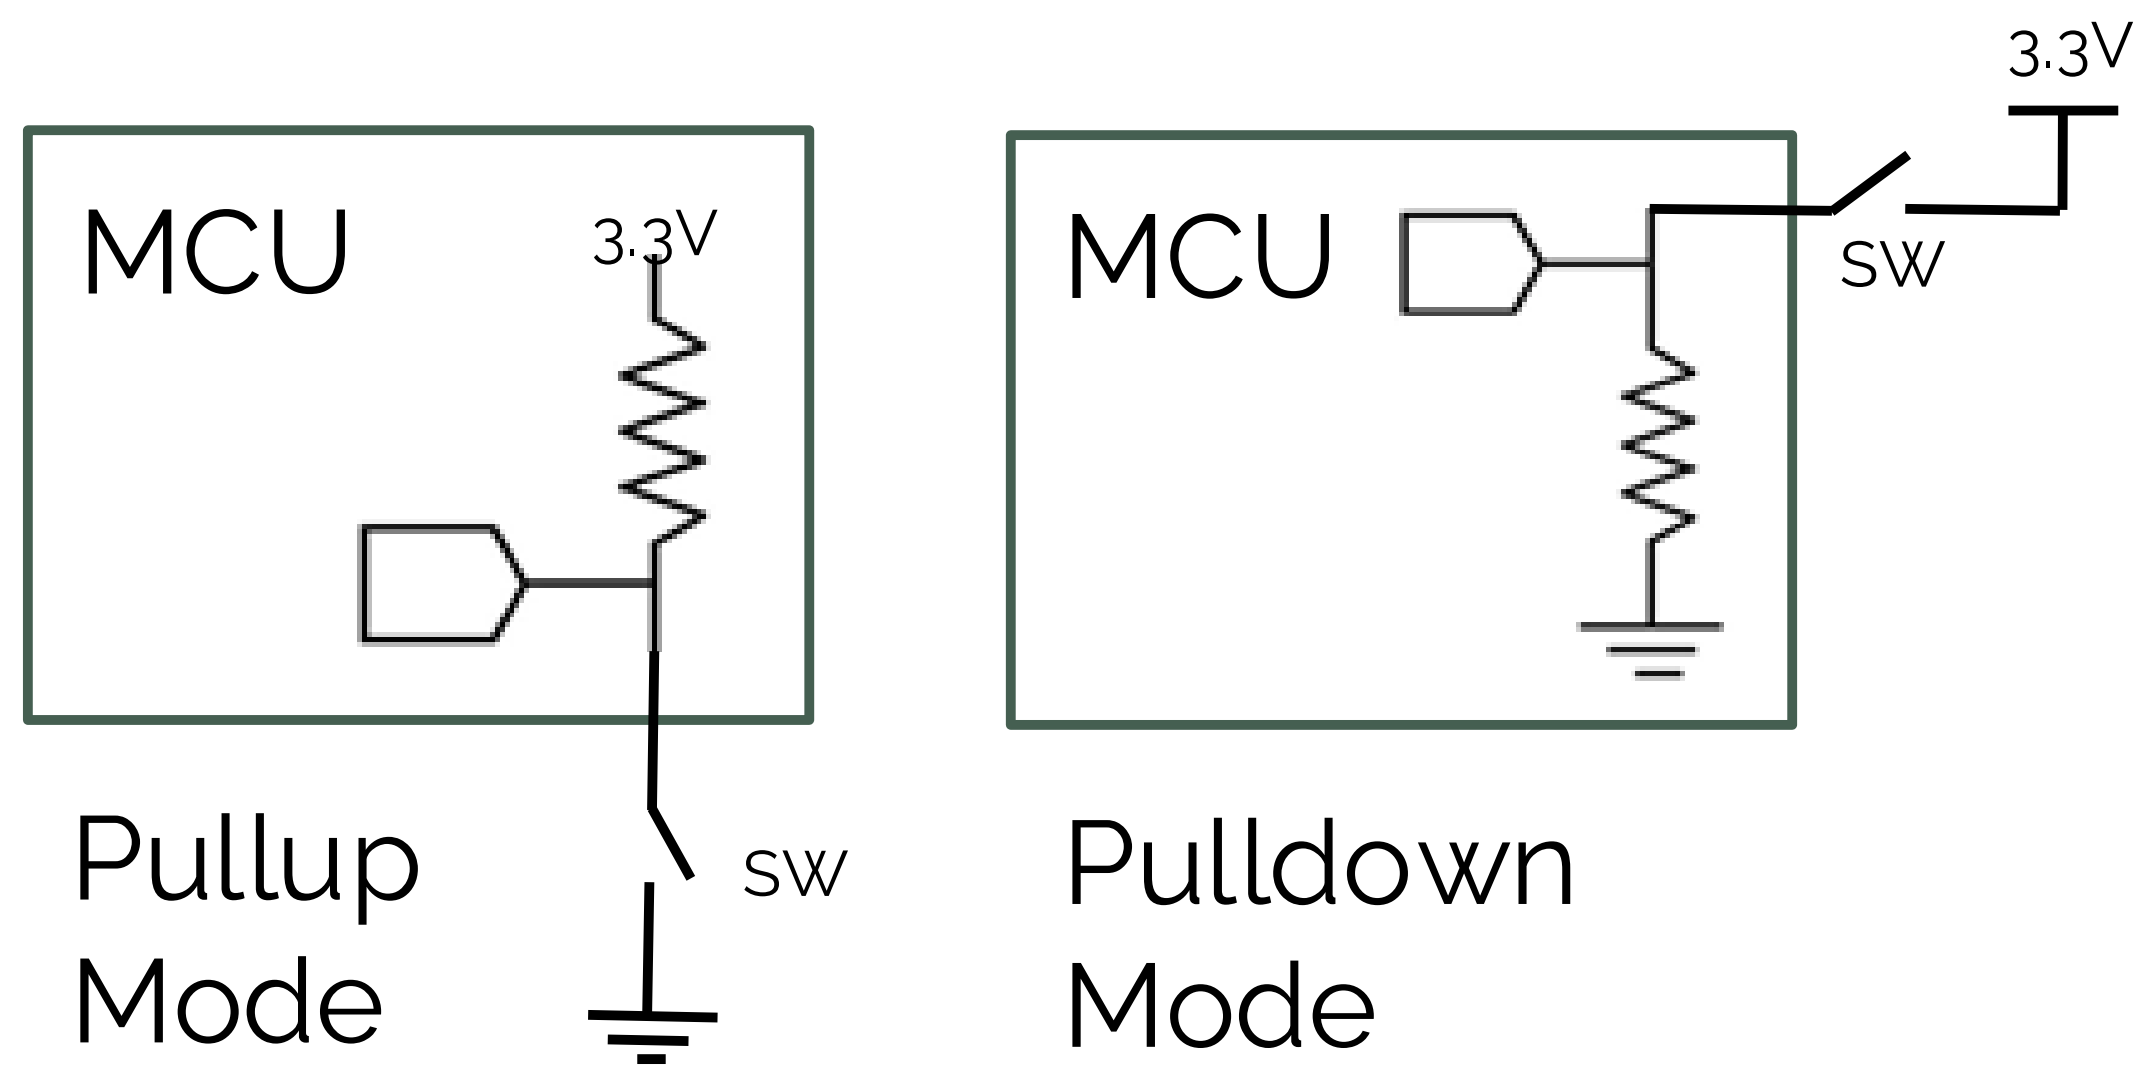
\includegraphics[width=0.5\linewidth]{img/image61.png}
\end{figure}
